\documentclass[10pt]{scrreprt}
\usepackage[a4paper, top=30mm, left=25mm, right=25mm, bottom=30mm]{geometry}
\usepackage[utf8]{inputenc}

%Options: Sonny, Lenny, Glenn, Conny, Rejne, Bjarne, Bjornstrup
\usepackage[Bjornstrup]{fncychap}
\usepackage{ngerman}
\usepackage{graphicx}
\usepackage{epstopdf}
\usepackage{etoolbox}
\usepackage{enumitem}
\usepackage{url}
\usepackage{numprint}
\usepackage{longtable}
\usepackage{tabu}
\usepackage{multirow}
\usepackage{caption}
\usepackage{array}
\usepackage{amssymb}

\makeatletter
\patchcmd{\@makechapterhead}{\vspace*{50\p@}}{\vspace*{-20\p@}}{}{}
\patchcmd{\@makeschapterhead}{\vspace*{50\p@}}{\vspace*{-20\p@}}{}{}
\makeatother

\newenvironment{details}[1][6pt]{%
  \parskip#1 \parindent6mm \raggedright%
  \def\item{\par\ignorespaces\hangindent=5mm \hangafter1}}{%
  \par\ignorespaces} 
  
\captionsetup[figure]{labelfont={sf,bf},textfont={sf}}
\deffootnotemark{[\thefootnotemark]}
\deffootnote{1.5em}{1em}{[\thefootnotemark] }
\setlength{\parindent}{0pt}
\renewcommand{\labelitemi}{ $\blacktriangleright$ }

\newcommand{\sfbf}[1]{\textbf{\sffamily #1}}
\newcommand{\sfit}[1]{\textit{\sffamily #1}}
\newcommand{\W}{\sfbf{W}}
\newcommand{\ziel}[1]{{\fontsize{9.5}{11}\textsf{/#1/}}}
\newcommand{\ziellabel}{Z}
\newcommand{\muss}{\renewcommand{\labelenumi}{\textbf{\ziel{\ziellabel\numprint{\theenumi}0}}}}
\newcommand{\wunsch}{\renewcommand{\labelenumi}{\textbf{\ziel{\ziellabel\numprint{\theenumi}0W}}}}
\newcommand{\JoglEarth}{\raisebox{-1.3mm}{
\includegraphics[scale=0.33]{Logo-Text.eps}} }
\newcommand{\textref}[1]{\mbox{\raisebox{0.1ex}{\small$\rightarrow$ }\textit{#1}}}

  

\begin{document}

\thispagestyle{empty}
\sffamily
 
\title{Pflichtenheft}

\begin{figure}
\begin{flushright}
	
\includegraphics[scale=0.4]{uniLogo.eps}
\vspace{2.0 cm}
\end{flushright}
\end{figure}

\begin{center}
\vspace{2.0 cm}
{\LARGE SEP – Wintersemester 2013/14}

\vspace{1.0 cm}
\textbf{{\Huge Pflichtenheft}}

\vspace{0.8 cm}
\begin{figure}[!htb]
\begin{center}
	%
\includegraphics[scale=1.0]{projektLogo.eps}
	
\includegraphics[scale=1.5]{Logo-Print.eps}
\end{center}
\end{figure}

\vspace{0.2 cm}
\textbf{{\huge OpenStreetMap: Die Welt in 3D}}

\vspace{1.5 cm}
25.10.2013

\vspace{0.5 cm}
Version: 1.0

\vspace{1.5 cm}
{\Large Projektbetreuer: Peter Barth}

\vspace{1.5 cm}
\begin{tabular}{|c|c|c|}
\hline 
\rule[-1ex]{0pt}{4ex} \textbf{Phase} & \textbf{Verantwortlicher} & \textbf{E-Mail Adresse} \\ 
\hline  \hline
\rule[-1ex]{0pt}{4ex} Pflichtenheft & Gabriele Haas & haasgab@fim.uni-passau.de \\ 
\hline  \hline
\rule[-1ex]{0pt}{4ex} Entwurf & Thomas Eder & ederthom@fim.uni-passau.de \\ 
\hline  \hline
\rule[-1ex]{0pt}{4ex} Spezifikation & Christof Blauberger & blauberg@fim.uni-passau.de \\ 
\hline  \hline
\rule[-1ex]{0pt}{4ex} Implementierung & Fabian Knorr & knorrfab@fim.uni-passau.de \\ 
\hline \hline 
\rule[-1ex]{0pt}{4ex} Testing & Constantin Wenger & wengerco@fim.uni-passau.de \\ 
\hline  \hline
\rule[-1ex]{0pt}{4ex} Präsentation & Sebastian Reichl & reichlse@fim.uni-passau.de \\ 
\hline 
\end{tabular}

\end{center}



\rmfamily
\tableofcontents



\chapter{Ausgangssituation}
Die Kartendaten des OpenStreetMap-Projekts erfreuen sich immer größerer Beliebtheit. Der Detailgrad der Daten, die Menge an verschiedenen Merkmalen und die Genauigkeit der Daten sind in den meisten Regionen der Welt ihrer Konkurrenz weit voraus. Durch die verschiedenartigen Karten, Kartenstile und Spezialanwendungen auf Basis von OpenStreetMap gibt es eine unzählige Menge von Anwendungsmöglichkeiten.

Außerdem ist die Grafikleistung einfacher Desktoprechner bereits für aufwändige 3D-Anwendungen ausgelegt. Die Vorlieben der Benutzer hat sich in den letzten Jahren dahingehend geändert, dass die visuelle Gestaltung wie auch die intuitive Bedienung ausschlaggebend für die Wahl eines Softwareproduktes ist.

\vspace{0.5cm}

Zwar existieren bereits ähnliche Softwarepakete, jedoch keines mit den folgenden Schwerpunkten:
\begin{itemize}
\item Primäre Verwendung von Kartendaten des OpenStreetMap-Projekts
\item Freie Wählbarkeit von Kartenquellen durch den Benutzer
\item Intuitive Bedienung ohne Einarbeitungszeit
\item Die Möglichkeit der spielerischen Benutzung durch Kinder ohne PC-Kenntnisse
\item Vollständige Plattformunabhängigkeit durch Java
\item Effiziente Speicher- und Bandbreitennutzung
\end{itemize}

\vspace{0.5cm}

Mit diesen Grundprinzipien soll eine 3D-Desktopanwendung basierend auf den Daten von OpenStreetMap und der NASA entworfen werden.




\chapter{Produkteinsatz}
\section{Anwendungsbereich}
Die Desktopanwendung \JoglEarth soll eine interaktive, dreidimensionale Ansicht der Welt auf Basis der freien Daten des OpenStreetMap-Projekt bieten. \\

Die grafische Benutzeroberfläche zeigt dafür eine Weltkugel, die frei gedreht und gezoomt werden kann. Die Steuerung erfolgt hierbei mit Tastatur und Maus. Die Oberflächentextur kann hierbei aus verschiedenen Typen wie Satellitenbildern der NASA oder Kartendaten des OpenStreetMap-Projekts gewählt werden. 
So besteht die Möglichkeit bis zu Straßenkarten zu zoomen und auch Städte oder andere Orte mit Hilfe einer Suchfunktion zu finden. \\

Es können auch weitere Anzeigeeinstellungen vorgenommen werden, wie eine freie Konfigurierbarkeit der Kartenserver oder das Einblenden von Overlays z.B. Banken, Tankstellen, Tierparks.  
Damit ist eine Anpassung der angezeigten Inhalte auf verschiedene Altersstufen und Interessengruppen möglich.


\section{Zielgruppe}
Primäre Zielgruppe des Systems sind Privatanwender, die eine andere Art der Kartendarstellung als die typischen Onlinekarten bevorzugen. \\

Auch soll die Anwendung wissbegierige Kinder ansprechen. Voraussetzung ist lediglich der geübte Umgang mit der Maus und/ oder Tastatur.

\section{Betriebsbedingungen}
\begin{itemize}
\item Bestehende dauerhafte Internetverbindung zum Laden des Kartenmaterials.
\item Nach der Abschlusspräsentation werden keine weiteren 
Veränderungen vorgenommen. Es erfolgt keine Wartung.
\end{itemize} 

\section{Sicherheit, Datenschutz}
Die Anwendung wahrt die Sicherheit des Systems und schützt die Privatsphäre des Nutzers.
\begin{itemize}
\item Es ist weder zur Bedienung, noch zum Beschaffen der Kartendaten eine Authentifikation erforderlich 
\item Es werden keine Persönlichen Daten des Anwenders über das Netz übertragen werden
\item Es wird kein Code aus dem Netz nachgeladen und ausgeführt
\item Das Programm hat keine (unter Umständen angreifbare) Serverfunktionalität
\end{itemize}


\section{Lizenzen}
Wird das Produkt veröffentlicht, so müssen die Lizenzen der verwendeten Bibliotheken und Datenquellen berücksichtigt werden:
\begin{itemize}
\item Teile der JOGL-Bibliothek sind unter mehreren Versionen der BSD-Lizenz, der SGI Free Software License und der Apache-Lizenz, der Ubuntu Font License und mehreren proprietären Lizenzen veröffentlicht. Details dazu finden sich bei  \footnote{\url{https://jogamp.org/git/?p=jogl.git;a=blob;f=LICENSE.txt}}.
\item OpenStreetMap ist „OpenData“ im Sinne der Open Data Commons Open Database Lizenz (ODbL). Die Kartografie der Kartenkacheln stehen unter der Linzenz  Creative Commons „Namensnennung, Weitergabe unter gleichen Bedingungen 2.0 (CC BY-SA). Weitere Infos, wie auch eine Vorgabe zum Hinweisen auf der Urheberschaft des OSM-Projekts finden sich bei \footnote{\url{http://www.openstretmap.org/copyright}}.
\item Die Daten der Overpass API stehen ebenfalls unter der ODbL.
\item Die Satellitenbilder der NASA sind frei verfügbar und stehen unter der Lizenz, die sich bei \footnote{\url{http://www.nasa.gov/audience/formedia/features/MP_Photo_Guidelines.html}} findet.
\item JGoodies Forms steht unter der BSD-Lizenz bei \footnote{\url{http://opensource.org/licenses/bsd-license.html}}.
\end{itemize}




\chapter{Produktumgebung}
\section{Software}
Da das Projekt auf Java setzt, ist es betriebssystemunabhängig. Es wird jedoch das Java Runtime Environment in Version 7 vorausgesetzt. Außerdem muss ein Fenstersystem und Netzwerkunterstützung zur Verfügung stehen. Zusätzliche Programmbibliotheken, die zum Ausführen des Softwarepakets nötig sind werden geliefert.\\

Da die Software von Seiten der Entwickler nur auf einem kleinen Teil der möglichen Umgebungen getestet werden kann, sollen mindestens folgende Konfigurationen unterstützt werden:
\begin{itemize}
\item Windows 7 und 8 auf x86{\_}64 mit den Herstellertreibern von nVidia und AMD
\item Linux auf x86{\_}64 mit X.org und proprietären Treibern von nVidia / AMD sowie den freien radeon-Treibern für AMD
\end{itemize}


\section{Hardware}
Wie auch bei der Software der Fall, sollte die Anwendung mit nahezu allen modernen Desktopsystemen kompatibel sein. Folgende Konfiguration wird jedoch für eine optimale Darstellung mindestens empfohlen:
\begin{itemize}
\item Dual-Core-Prozessor mit 1 GHz Taktfrequenz
\item 2 Gigabyte RAM
\item 200 Megabyte freier Speicherplatz
\item Grafikkarte: Onboard-Grafik mit OpenGL 2.0-Unterstützung
\item Bildschirm mit 1024x768 Pixeln Auflösung und 24 Bit Farbtiefe
\item Standard-Tastatur und Maus
\end{itemize}



\section{Orgware}
Zum Laden der Kartendaten wird eine durchgehende Internetverbindung benötigt. Um die Wartezeiten akzeptabel zu halten wird mindestens 1MBit/s empfohlen.




\chapter{Zielbestimmungen}

\section{Musskriterien}
\begin{itemize}
\item Intuitiv bedienbare, grafisch ansprechende GUI mit einklappbarer Seitenleiste und Sprachunterstützung für Englisch und Deutsch (siehe \ziel{F010}, \ziel{F020}, \ziel{F030}, \ziel{F040})
\item Bedienung mit Maus und Tastatur (siehe \ziel{F160})
\item Anzeige der momentanen und der möglichen Zoomstufen (siehe \ziel{F050})
\item Sinnvolle Beschränkung der Zoomstufen und Beweglichkeit (siehe \ziel{F210})
\item Ladebalken für im Hintergrund geladene Kartendaten (siehe \ziel{F060})
\item Felder zur Anzeige und zur Änderung des Längen- und Breitengrads (siehe \ziel{F070})
\item Anzeige des momentanen Kartenmaßstabs (siehe \ziel{F080})
\item Ansichtsmodus wechselbar zwischen 3D-Globus und flache Kartenansicht (siehe \ziel{F090})
\item Kartenmaterial wechselbar zwischen Satellitenbildern und OpenStreetMap (siehe \ziel{F110})
\item Drehen, Kippen, Zoomen der Ansichten (siehe \ziel{F170}, \ziel{F180})
\item Text- und Symboloverlays für Städte und POIs, Anzeige der Details dazu im Detailfenster (ohne Markierung und Speicherfunktion) (siehe \ziel{F200}, \ziel{F220}, \ziel{F350}, \ziel{F380})
\item Beschränkung der Anzahl gleichzeitig geladener Overpass-Einträge (siehe \ziel{F240})
\item Effizientes Laden der Kartendaten (siehe \ziel{F250}, \ziel{F260}, \ziel{F270}, \ziel{F280}, \ziel{F290}, \ziel{F300}, \ziel{F330W})
\end{itemize}

\section{Wunschkriterien}
\begin{itemize}
\item Kinder-Weltkarte (siehe \ziel{F100W})
\item Sonnensystem-Modellansicht als weiteren Ansichtsmodus (siehe \ziel{F100W}, \ziel{F130W})
\item Sternenhimmel als Hintergrund (siehe \ziel{F140W})
\item Ansichtseinstellungen können gespeichert werden (siehe \ziel{F400W})
\item 3D-Höhenprofil (siehe \ziel{F120W})
\item 3D-Modelle für Häuser/Bäume (siehe \ziel{F120W}, \ziel{F230W})
\item Punkte markieren mit Notiz und Speicherfunktion (siehe \ziel{F190W}, \ziel{F230W}, \ziel{F360W}, \ziel{F390W}, \ziel{F400W})
\item Suchfunktion für Overpass-Einträge, Lokal/Global (siehe \ziel{F370W})
\item Nur rendern wenn nötig (bei Bildänderung) (siehe \ziel{F340W})
\item Grafikeinstellungen wie Antialiasing oder Texturfilterung (siehe \ziel{F150W})
\item Platzhaltertextur für nicht verfügbare Kacheln (siehe \ziel{F310W})
\item Vorausladen von Kartendaten an den Rändern der Anzeige (siehe \ziel{F320W})
\end{itemize}

\section{Abgrenzungskriterien}
\begin{itemize}
\item Keine Druck / Speicherfunktion für Kartenmaterial
\item Kein Export für markierte Punkte (Speicherfunktion in externe Datei)
\item Keine dynamischen Flüsse oder andere Animationen
\item Keine Routenplanung
\item Keine Unterstützung für andere Eingabegeräte wie Joysticks
\item Kein Login oder Authentifizierung um Zugriff auf vom Benutzer gespeicherte Markierungen zu erhalten.
\end{itemize}


\chapter{Benutzeroberfläche}

\section{Visuelles Konzept}

\begin{itemize}
	\item Das Hauptelement der Benutzeroberfläche ist die Karten- oder Globusansicht, die sich im rechten Fensterteil befindet. Der sichtbare Kartenausschnitt kann interaktiv mit Maus oder Tastatur verschoben werden.
	\item Im 2D-Modus zeigt die Ansicht eine Projektion der Karte auf die Ebene, die in der Ansicht nach links/rechts und oben/unten verschoben sowie (perspektivisch) gekippt werden kann.
	\item Im 3D-Modus wird ein Globus gezeigt, auf den das Kartenmaterial projiziert wird. Die Ansicht kann um die Erdachse sowie in Richtung der Pole gedreht; ab einem gewissen Zoomlevel am Kameraursprung gekippt werden.
	\item Am linken Rand des Fensters befindet sich eine Seitenleiste, die sämtliche Steuerungsfunktionen bereitstellt. Der obere Teil ist in Tabs unterteilt, mit denen Funktionen gruppiert werden; der untere Teil zeigt Details zum momentan zentrierten Punkt an.
\end{itemize}


\vspace{1cm}
\begin{figure}[h]
	\centering
	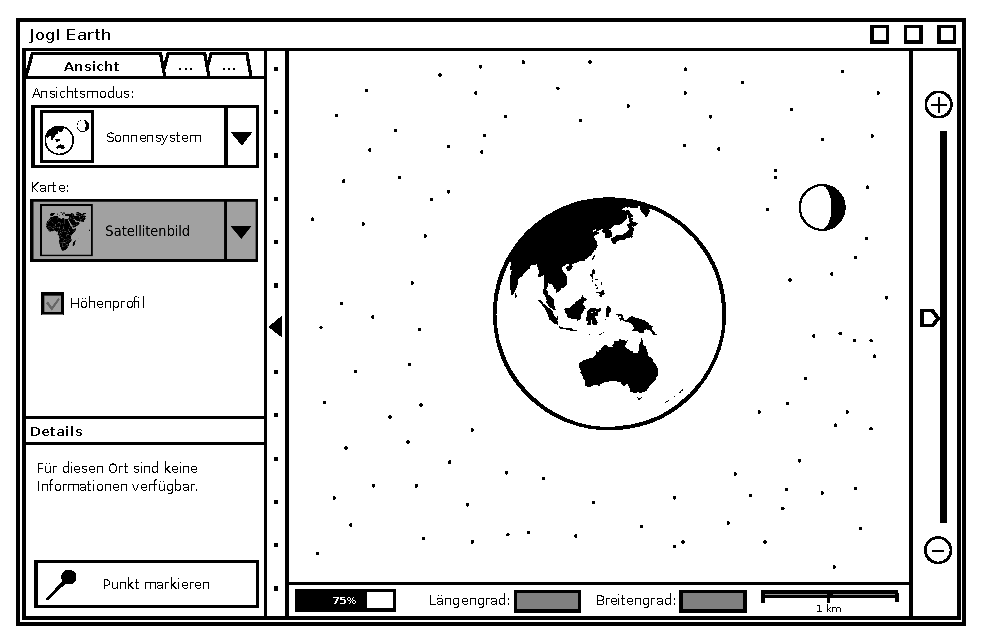
\includegraphics[scale=0.9]{GUI-Sonnensystem.eps}
	\caption{Die Benutzeroberfläche mit geöffnetem Ansichts-Tab im Sonnensystemmodus}
\end{figure}

\begin{figure}
	\centering
	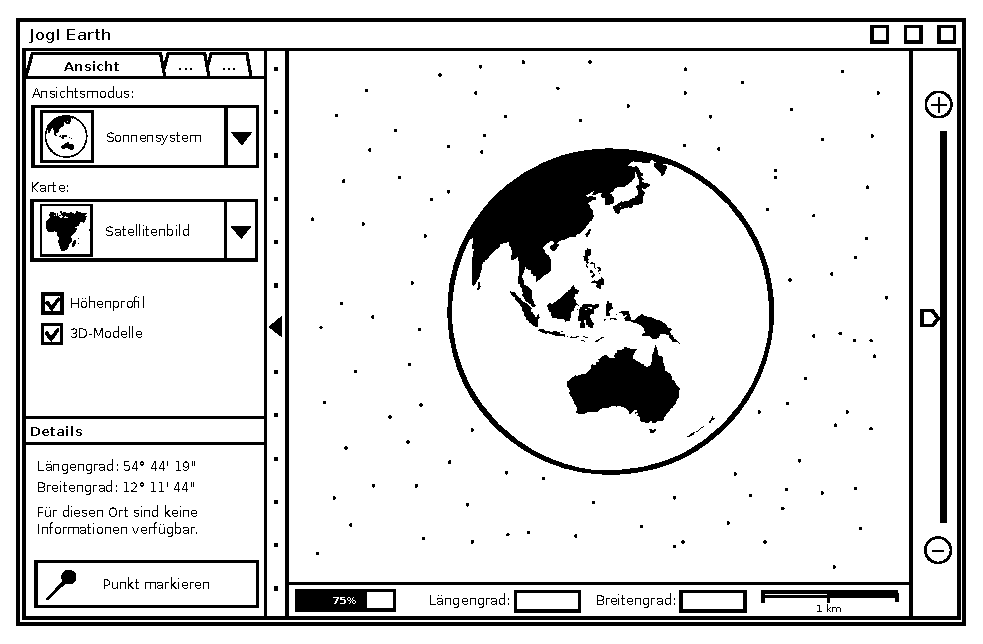
\includegraphics[scale=0.9]{GUI-Ansicht.eps}
	\caption{Die Benutzeroberfläche mit geöffnetem Ansichts-Tab mit dargestelltem Globus}
\end{figure}

\begin{figure}
	\centering
	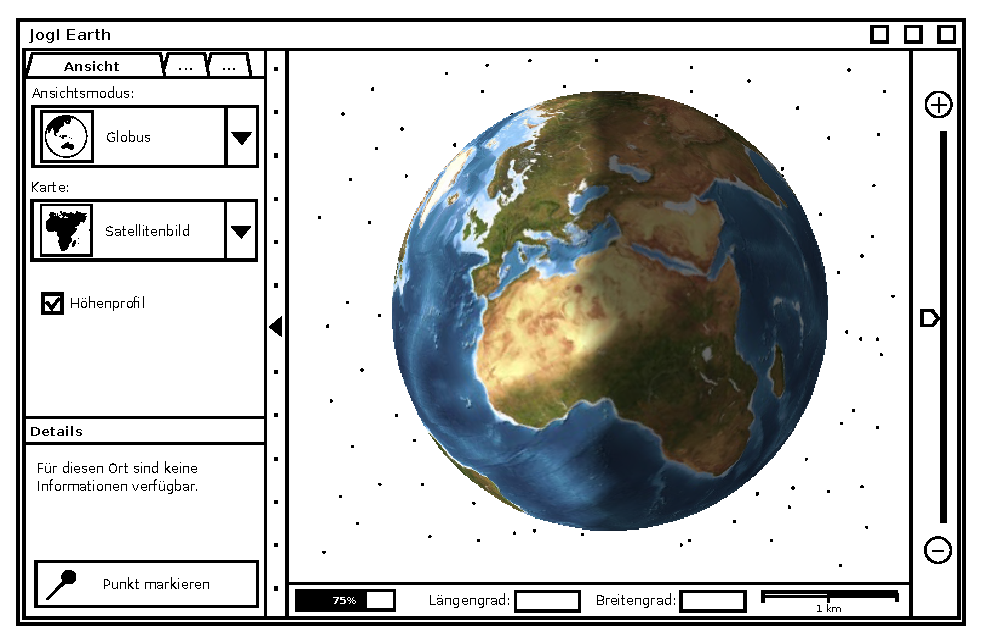
\includegraphics[scale=0.9]{GUI-Ansicht-Welt.eps}
	\caption{Die Benutzeroberfläche mit der Ansicht auf die Weltkugel}
\end{figure}
\begin{figure}
	\centering
	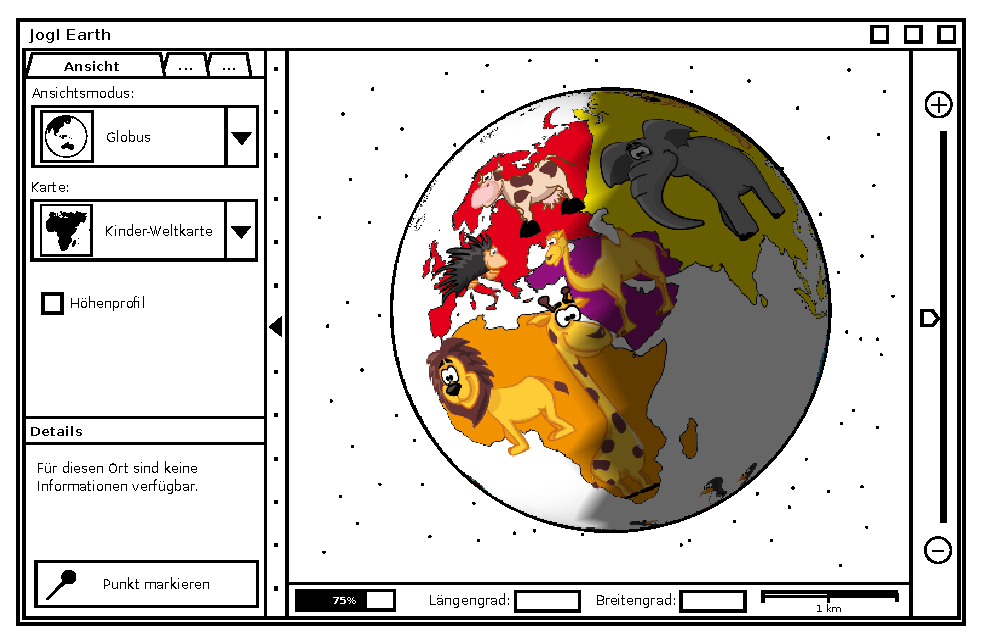
\includegraphics[scale=0.9]{GUI-Ansicht-Kinder-Weltkarte.eps}
	\caption{Die Benutzeroberfläche mit der Kinder-Weltkarte}
\end{figure}
\begin{figure}
	\centering
	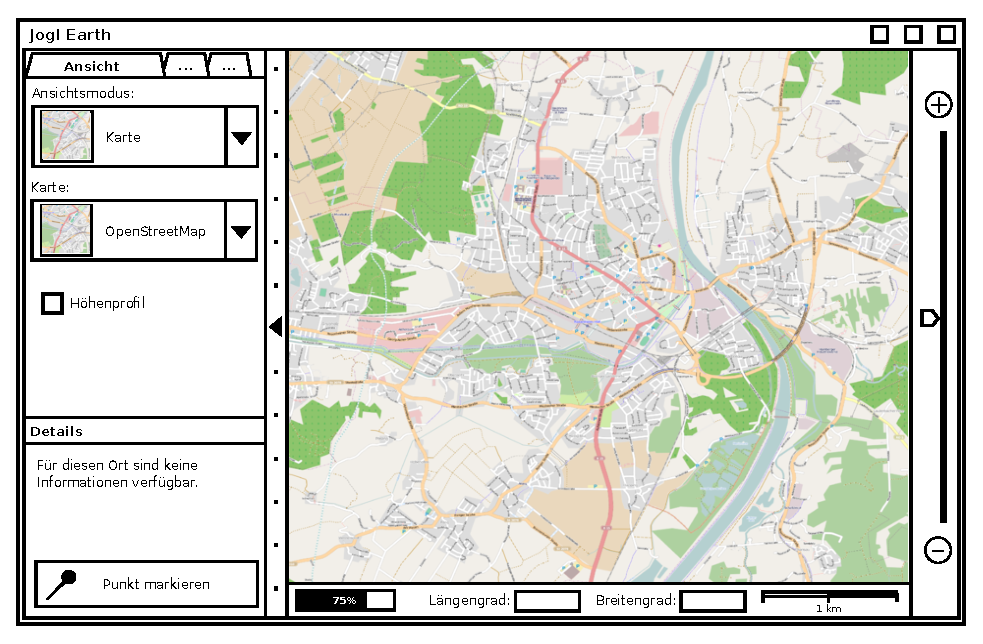
\includegraphics[scale=0.9]{GUI-Ansicht-Strassenkarte.eps}
	\caption{Die Benutzeroberfläche mit der Ansicht auf eine Straßenkarte}
\end{figure}

\begin{figure}
	\centering
	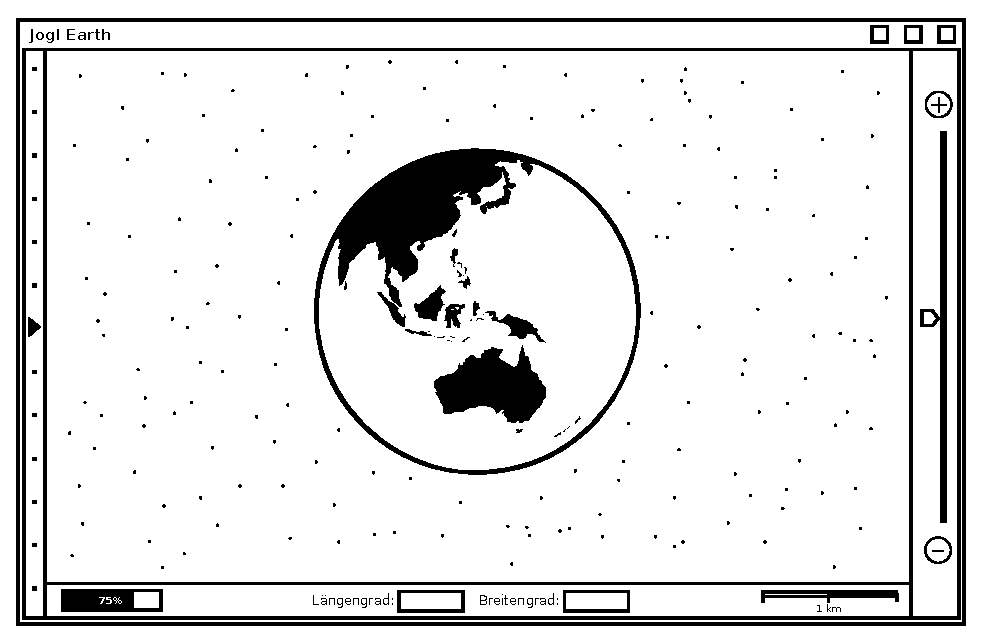
\includegraphics[scale=0.9]{GUI-Ausgeblendet.eps}
	\caption{Die Benutzeroberfläche mit ausgeblendeter Einstellungsleiste}
\end{figure}
\begin{figure}
	\centering
		\begin{minipage}[c]{6cm}
        \centering
                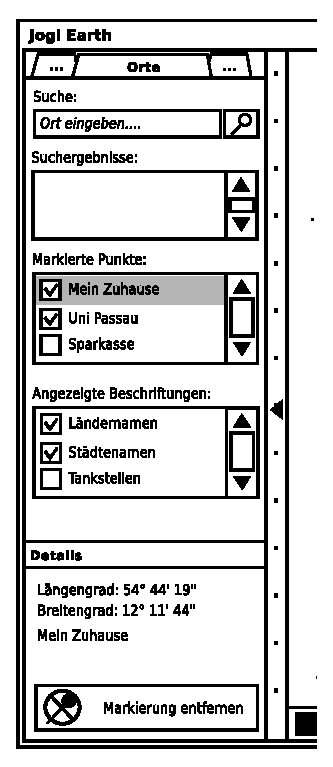
\includegraphics[scale=0.9]{GUI-Orte.eps}
        \end{minipage}
        \begin{minipage}[c]{6cm}
        \centering
                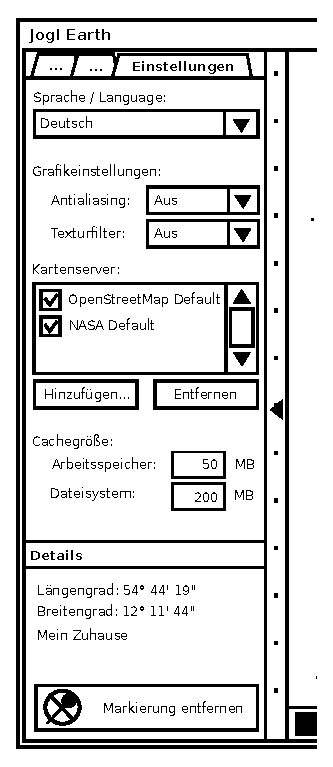
\includegraphics[scale=0.9]{GUI-Einstellungen.eps}
        \end{minipage}
        \caption{Der Orte- und der Einstellungstab}
\end{figure}
\begin{figure}
	\centering
	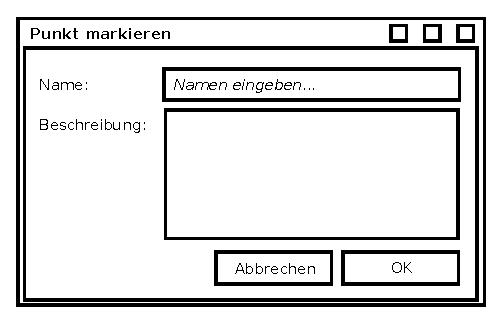
\includegraphics[scale=0.9]{GUI-Markieren.eps}
	\caption{Das Dialogfenster zur Eingabe der Beschreibung beim Markieren eines Punktes}
\end{figure}

\clearpage
\pagebreak

\section{Steuerung der Kartenansicht}

\subsection{Mausbelegung}
\vspace{3mm}
\begin{center}
\begin{tabular}{|>{\centering \arraybackslash}m{3cm}|m{9cm}|}
\hline 

\rule[-1ex]{0pt}{4ex} \sffamily\textbf{Tastenbelegung} &\rule[-1ex]{0pt}{4ex} \sffamily\textbf{Bedeutung} \\ 
\hline
\hline

\includegraphics[scale=1.0]{KeyImages/mouseDrag_left.eps} & Drehen der Erdkugel / Verschieben der Karte \\ 
\hline 

\includegraphics[scale=1.0]{KeyImages/mouseDoubleClick_left.eps} & Punkt markieren und im Kartenfenster zentrieren \\
\hline

\includegraphics[scale=1.0]{KeyImages/mouseDrag_right.eps} & Kippen der Karte \\
\hline

\includegraphics[scale=1.0]{KeyImages/mouse_scrollen.eps} & Zoomen der Ansicht \\
\hline
\end{tabular} 
\end{center}




\vspace{5mm}
\subsection{Tastaturbelegung}
\vspace{3mm}
\begin{center}
\begin{tabular}{|>{\centering \arraybackslash}m{3cm}|m{9cm}|}
\hline 
\sffamily \rule[-1ex]{0pt}{4ex} \textbf{Tastenbelegung} & \sffamily \rule[-1ex]{0pt}{4ex} \textbf{Bedeutung} \\
\hline 
\hline
\rule[-1ex]{0pt}{7ex}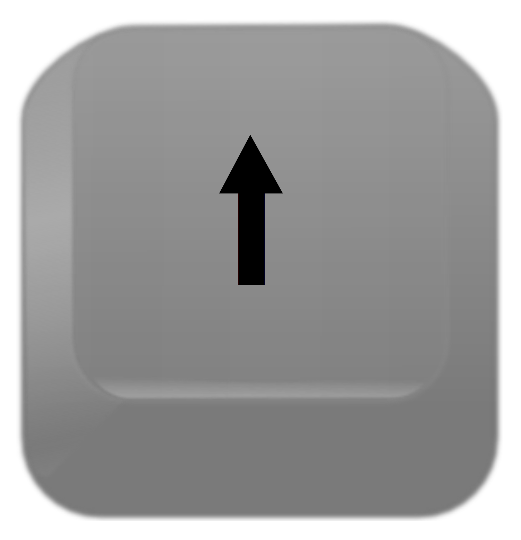
\includegraphics[scale=0.08]{KeyImages/key_arrow_up.eps}& \multirow{3}{*}{Drehen der Erdkugel, Verschieben der Karten}\\
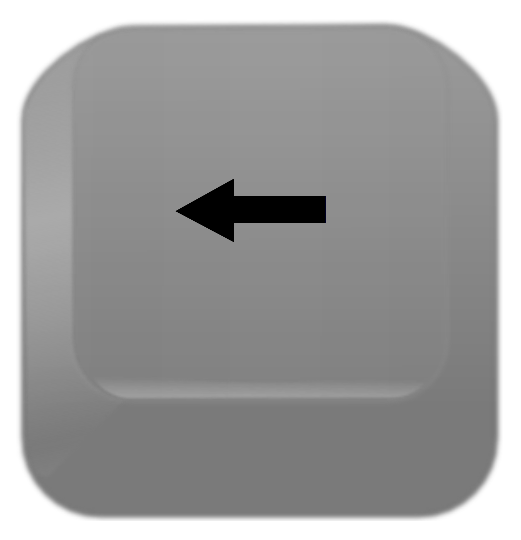
\includegraphics[scale=0.08] {KeyImages/key_arrow_left.eps} 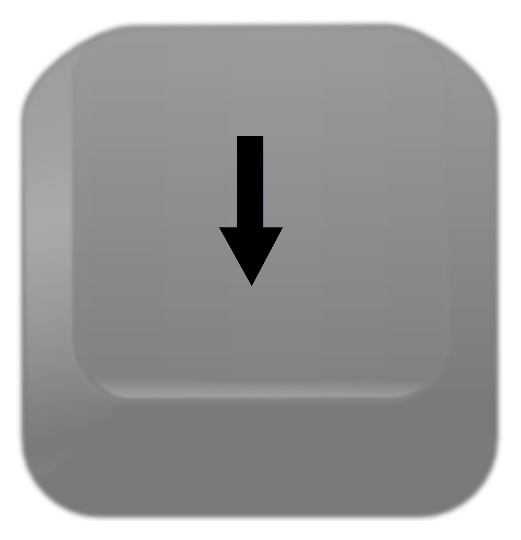
\includegraphics[scale=0.08]{KeyImages/key_arrow_down.eps} 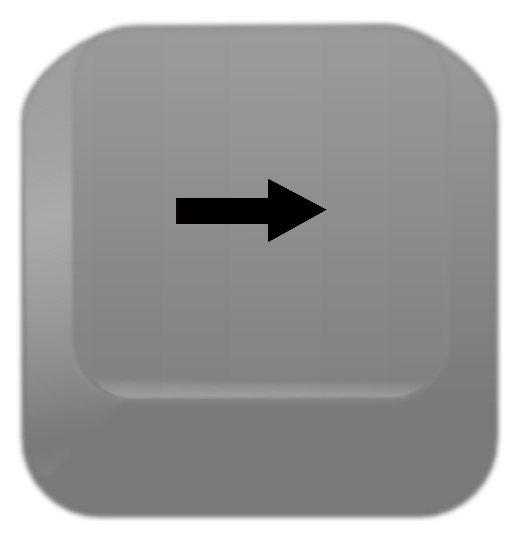
\includegraphics[scale=0.08]{KeyImages/key_arrow_right.eps} &  \\
\hline
\rule[-1ex]{0pt}{7ex} 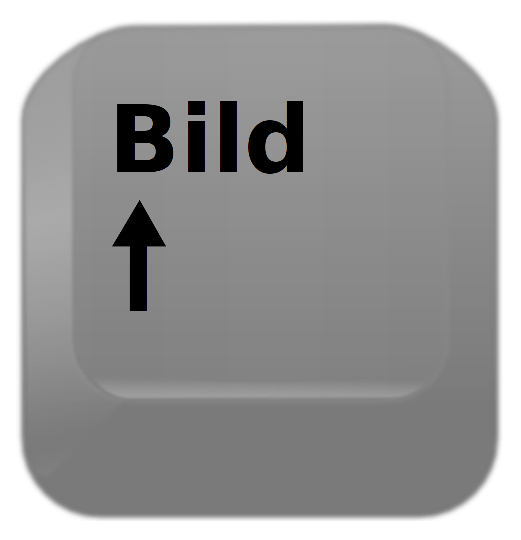
\includegraphics[scale=0.08]{KeyImages/key_Bild_Auf.eps}  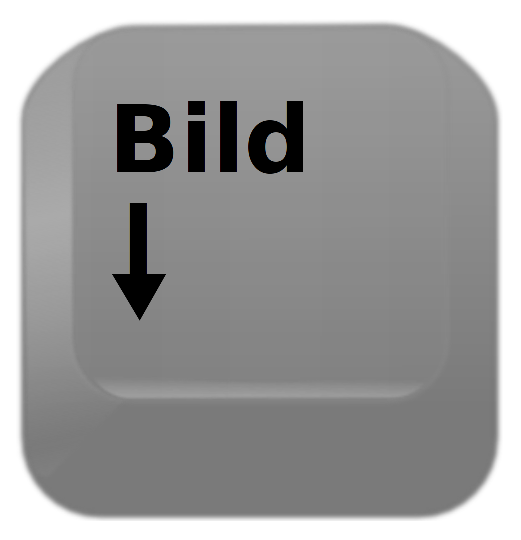
\includegraphics[scale=0.08]{KeyImages/key_Bild_Ab.eps} & Kippen der Karte \\
\hline
\rule[-1ex]{0pt}{7ex} 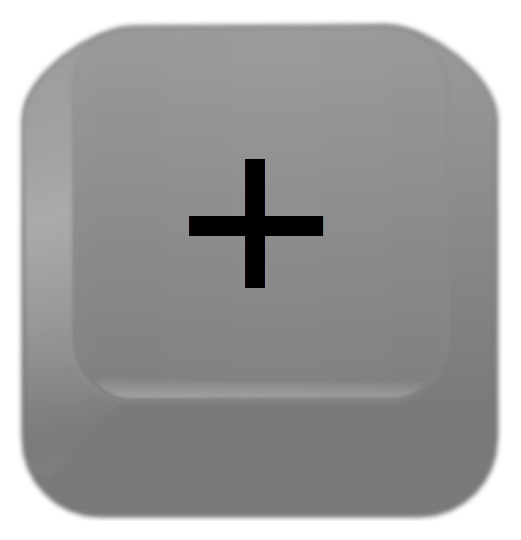
\includegraphics[scale=0.08]{KeyImages/key_Plus.eps}  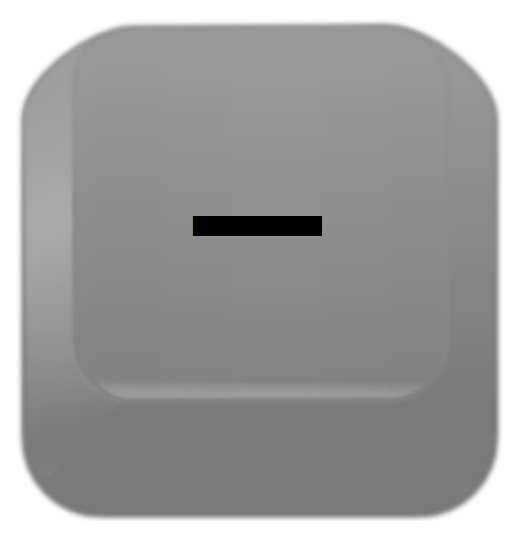
\includegraphics[scale=0.08]{KeyImages/key_Minus.eps} & Zoomen der Ansicht \\
\hline
\rule[-1ex]{0pt}{7ex} 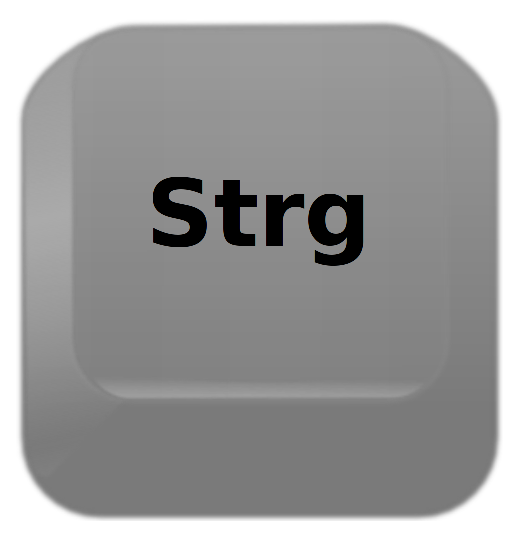
\includegraphics[scale=0.08]{KeyImages/key_Strg.eps} \rule[-1ex]{0pt}{7ex} \textbf{+} 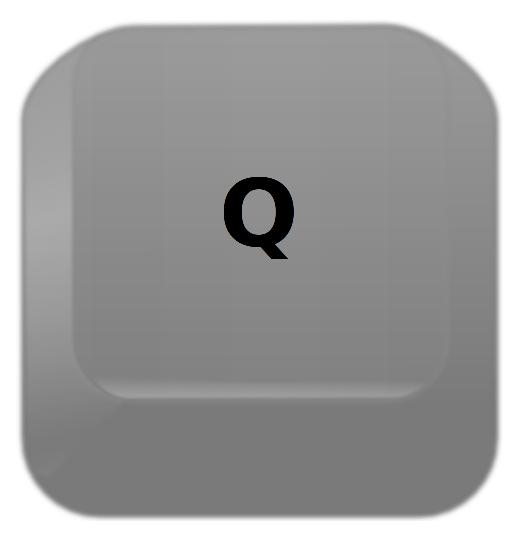
\includegraphics[scale=0.08]{KeyImages/key_Q.eps} & Beenden der Anwendung und Schließen der GUI \\ 
\hline
\end{tabular} 
\end{center}




\chapter{Systemarchitektur}
Die Systemarchitektur folgt dem Model-View-Controller-Pattern.
\vspace{3mm}
\begin{figure}[h]
\centering
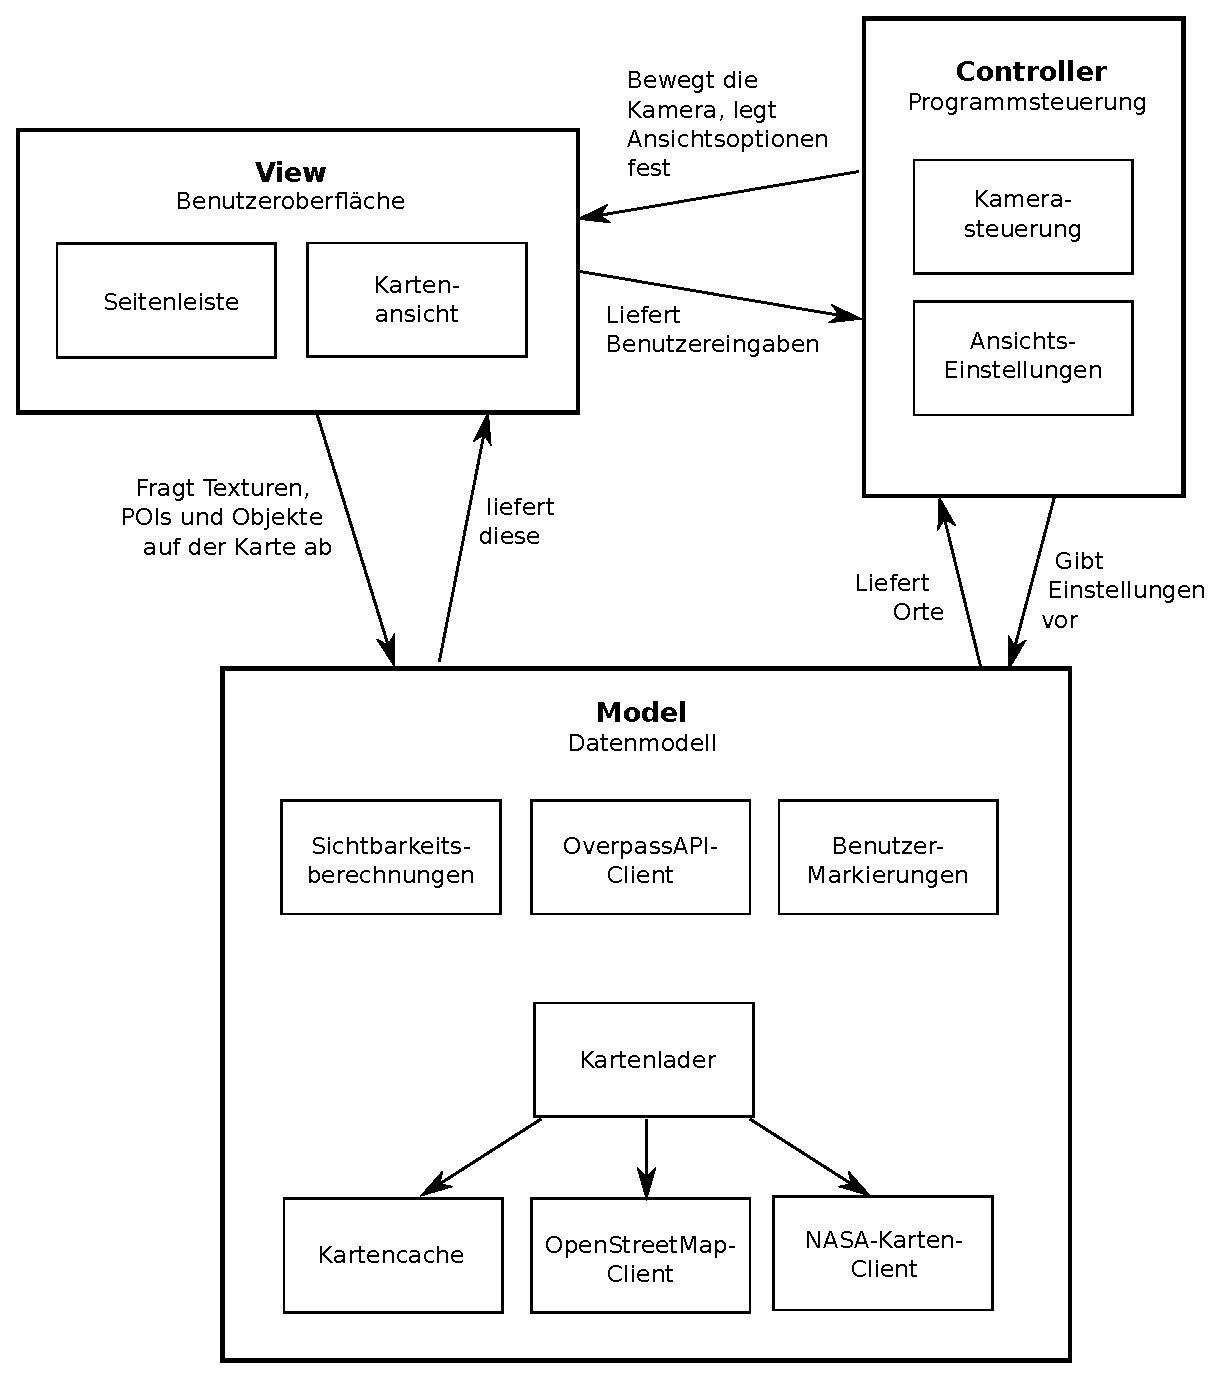
\includegraphics[scale=0.6]{ModelViewController.eps}
\caption{Konzept der Systemarchitektur (Abriss)}
\end{figure}
\subsubsection*{Controller}
Die \textbf{Programmsteuerung} übernimmt die Verarbeitung der Ein- und Ausgaben und steuert die Ansicht.
 Sie ist für die Umsetzung der Nutzerbefehle und gespeicherter Einstellungen verantwortlich.
\subsubsection*{View}
Die \textbf{Benutzeroberfläche} dient als Schnittstelle zwischen Anwender und Programm. Sie erzeugt eine visuelle Darstellung aus den Befehlen der Programmsteuerung und den Daten des Modells. Eingaben wie Tastendrücke oder das Anwählen eines GUI-Elements leitet sie an die Steuerung weiter.

\subsubsection*{Model}
Das \textbf{Datenmodell} ist dafür zuständig, Berechnungen und Anfragen bezüglich der Karte oder des Globus zu beantworten. Es bestimmt die Sichtbarkeit von Kartenabschnitten und beschafft Karten-, Markierungs- sowie ortsspezifische Daten.


\chapter{Produktfunktionen}

\nplpadding{2}
\muss
\renewcommand{\ziellabel}{F}

Wunschkriterien werden mit {\W } gekennzeichnet, alle verbleibenden sind Musskriterien.

\section{Fensterverhalten}
\begin{enumerate}[leftmargin=2.2cm]
\item Das Programmfenster startet mit einer Größe von 1024x768 Pixeln. Die Größe ist mit 800x600 Pixeln nach unten, aber nicht nach oben beschränkt und kann vom Benutzer durch Vergrößern bzw. Verkleinern der GUI geändert werden.
\item Über den Fenstermanager (die Schließen-Funktion des Fensters) oder mit einem Tastenkürzel wird die Anwendung ohne Rückfrage beendet.
\item Die Einstellungsleiste am linken Rand der GUI ist einklappbar.
\item Auswahlmöglichkeit der Sprache: Englisch oder Deutsch
\end{enumerate}

\section{GUI-Elemente zur Navigation}
\begin{enumerate}[leftmargin=2.2cm,resume]
\item Das Zoomlevel kann über einen Schieber angezeigt und geändert werden.
\item Ein Ladebalken zeigt den Fortschritt der im Hintergrund geladenen Kartendaten an.
\item Der Längen- und Breitengrad des Punktes in der Bildschirmmitte wird über Eingabefelder angezeigt, und können geändert werden.
\item Der Maßstab des Punktes unter dem Anzeigemittelpunkt wird in einem Feld angezeigt.
\end{enumerate}

\section{Ansichtseinstellungen}
\begin{enumerate}[leftmargin=2.2cm,resume]
\item Es kann zwischen 3D- (Globus) und 2D-Ansichten (Aufsicht) gewählt werden.
\wunsch
\item Zusätzliche Ansichten bieten der Sonnensystemmodus und die Kinder-Weltkarte.
\muss
\item Es besteht eine Auswahl aus verschiedenen Kartentypen; wie Satellitenbildern und Straßenkarten.
\wunsch
\item Es sind Höhenprofile, sowie 3D-Ansichten von Häusern und 
Bäumen zuschaltbar.
\item Im Sonnensystemmodus werden zusätzliche Himmelskörper wie Sonne und Mond sichtbar, dafür ist die Zoommöglichkeit stark begrenzt und die Auswahlmöglichkeiten in der GUI sind stark eingeschränkt.
\item Ein Sternenhimmel als Hintergrundbild soll zuschaltbar sein.
\item Grafikeinstellungen wie Antialiasing oder Texturfilterung
\end{enumerate}

\section{Kartenansicht}
\begin{enumerate}[leftmargin=2.2cm,resume]
\item Die Kartenansicht kann interaktiv mit Maus und Tastatur bedient werden.
\item Im 2D-Kartenmodus kann die Ansicht nach links/rechts und oben/unten verschoben sowie (perspektivisch) gekippt werden. 
\item Im 3D-Kartenmodus kann die Ansicht um die Erdachse sowie in Richtung der Pole gedreht; ab einem gewissen Zoomlevel am Kameraursprung gekippt werden.
\wunsch
\item Im 2D-Kartenmodus kann der Benutzer Punkte markieren und speichern.
\muss
\item Im Detailfenster werden Informationen zum markierten Punkt angezeigt. Bei POIs sind das Adresse sowie Beschreibung; bei anderen Punkten genauer Längen- und Breitengrad.
\end{enumerate}

\section{Kartendarstellung}
\begin{enumerate}[leftmargin=2.2cm,resume]
\item In 3D-Darstellung kann die Ansicht nicht über die Pole hinweg gedreht werden, sodass die Pole im Fenster immer nach oben oder unten zeigen. Weiters wird das Zoomlevel beschränkt.
\item Overlays wie Städtenamen oder Symbole für Tankstellen werden als zweidimensionale Objekte an die Stelle der Anzeigefläche projiziert, an der der markierte Punkt auf dem Bildschirm erscheint.
\wunsch
\item Dreidimensionale Objekte wie Häusermodelle, Bäume, oder  Markierungen von Punkten werden direkt in die Szene eingefügt.
\muss
\item Die Menge der Angezeigten Overlays und 3D-Modelle wird beschränkt, sodass die Leistung wie auch die Lesbarkeit von Beschriftungen akzeptabel bleibt.
\end{enumerate}

\section{Laden der Kartendaten}
\begin{enumerate}[resume,leftmargin=2.2cm]
\item Das Laden von Kacheln geschieht über HTTP.
\item Welche Kacheln geladen werden müssen, wird  aus den sichtbaren Kartenabschnitten und dem momentanen Zoomlevel bestimmt.
\item Es werden nur die benötigen Karten für den jeweiligen Ausschnitt geladen.
\item Ist die Textur einer Kachel bereits geladen, wird sie direkt angezeigt.
\item Ist sie lokal nicht vorhanden, wird sie über einen passenden Kachelserver nachgeladen und dem Cache hinzugefügt.
\item Das Laden von Kacheldaten erfolgt im Hintergrund, während die Ansicht weiter gerendert werden kann.
\wunsch
\item Ist eine Textur noch nicht geladen oder nicht verfügbar, wird sie zwischenzeitlich durch eine Platzhaltertextur ersetzt.
\item Es werden zusätzliche Kacheln der direkten Randbereiche außerhalb der Ansicht geladen.
\item Ist die Textur einer Kachel noch nicht geladen wird zuerst versucht sie aus dem Cache im Arbeitsspeicher, dann aus dem Cache im Dateisystem zu laden. Die Cachegröße kann jeweils vom Benutzer angepasst werden.
\item Rendervorgänge sollen nur bei Bildänderungen gestartet werden
\end{enumerate}



\section{Orte}
\begin{enumerate}[leftmargin=2.2cm,resume]
\item Städtenamen, Points of Interest und andere Informationen können unter einer Vielzahl an Overlays an- und abgewählt werden.
\wunsch
\item Eigene Punkte können auf der Karte markiert, die Markierungen ein-/ausgeblendet, in einer Liste verwaltet und wieder entfernt werden. 
\item Orte und POIs können mittels einer Suchfunktion aufgefunden, angezeigt und den markierten Punkten hinzugefügt werden. Es kann dabei entweder im momentanen Kartenausschnitt oder global gesucht werden.
\end{enumerate}

\section{Detailfenster}
\begin{enumerate}[leftmargin=2.2cm,resume]
\item Das Detailfenster bietet die Möglichkeit nähere Informationen zu einem Punkt auf der Karte zu erhalten, wie zugehörigem Längen- und Breitengrad.
\wunsch
\item Der momentan in der Kartenansicht gewählte Punkt kann markiert,  gespeichert und falls bereits eine Markierung besteht wieder entfernt werden.
\item POI's sowie gewisse Einstellungen werden in einer Datei gespeichert, die bei Programmstart geladen wird.
\end{enumerate}



\chapter{Produktdaten}

\renewcommand{\ziellabel}{D}
\muss

Wunschkriterien werden mit {\W } gekennzeichnet, alle verbleibenden sind Musskriterien.\\

\vspace{5mm}

\begin{enumerate}[leftmargin=2cm]
\item Alle Daten des Programms werden im Verzeichnis der JAR-Datei (oder falls extra angegeben in einem Unterordner) abgelegt.
\item Es werden alle benötigten Bibliotheken mitgeliefert, das sind im einzelnen: 
\begin{itemize}
\item JOGL mit allen betriebssystemabhängigen Bibliotheken
\item die Apache HTTP Client Library
\item die Forms-Bibliothek von JGoodies.
\end{itemize}
\wunsch
\item Einstellungen werden in einer Datei \texttt{settings} gespeichert, die mit den Vorgabeeinstellungen dem Programm beiliegt. Zu den gespeicherten Daten gehören:
\begin{itemize}
\item Sprache
\item Antialiasing und Texturfilter
\item die verfügbaren und momentan gewählten Kartenserver
\item Eingestellte Puffergrößen
\item der zuletzt ausgewählte Ansichtsmodus, die gewählte Karte, Overlays und Ansichtsoptionen wie 3D-Modelle
\item Markierte Punkte mit Name und Notiz
\end{itemize}
\muss
\item Mitgelieferte Texturen wie beispielsweise die Kinder-Weltkarte oder Symbole für POIs liegen im Ordner \texttt{textures}.
\begin{figure}[!htb]
	\centering
	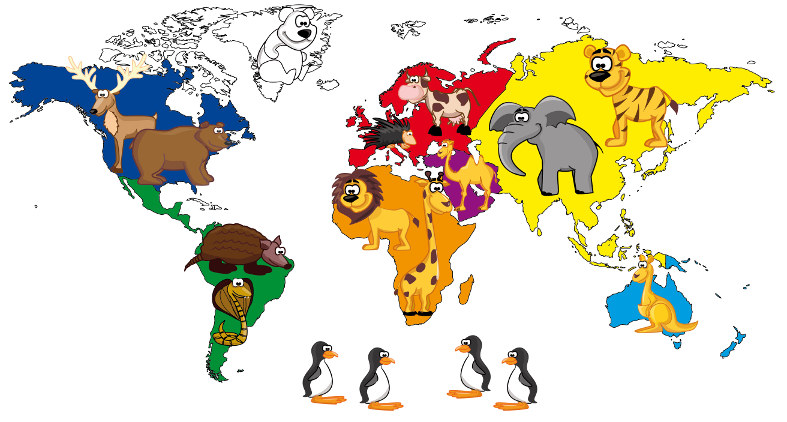
\includegraphics[scale=0.3]{Kinder-Weltkarte.jpg}
\end{figure}
\item Zwischengespeicherte Kacheln werden im Ordner \texttt{cache} abgelegt. Dabei erhält jede Kombination aus Server- und Kartentyp ein eigenes Unterverzeichnis.
\end{enumerate}


\chapter{Produktleistungen}

\renewcommand{\ziellabel}{L}
\muss

Wunschkriterien werden mit {\W } gekennzeichnet, alle verbleibenden sind Musskriterien.

\begin{enumerate}[leftmargin=2.2cm]
\item Die Benutzeroberfläche soll grafisch ansprechend, gut strukturiert und intuitiv verständlich gehalten sein.
\wunsch
\item Um auch Kinder zu motivieren, Jogl Earth zu verwenden, wird eine altersgemäße Kinder-Weltkarte mit ausgeliefert.
\muss
\item Die Oberfläche wird in den Sprachen Englisch und Deutsch angeboten.
\item Die gesamte GUI ist komfortabel mit Maus und Tastatur steuerbar.
\item Die einklappbare Seitenleiste in der GUI soll dem Benutzer die Möglichkeit bieten, 3D- und 2D-Ansichten in einem größeren Umfang (flächig) darzustellen.
\item Die Bewegung der Kamera und das Anpassen des Zoomlevels wird beschränkt, damit keine Darstellungsfehler wie das Durchdringen der Kartenebene auftreten.
\item Die Menge der angezeigten Overlays und 3D-Modelle wird beschränkt, sodass die Leistung wie auch die Lesbarkeit von Beschriftungen gegeben ist.
\item Eine weitere Option für den Benutzer soll das Markieren von Punkten bzw. Orten in den Karten darstellen. Diese sollen gespeichert und mit Namen und Notizen versehen werden können.
\item Zudem soll eine Suchfunktion den Nutzer unterstützen, die POIs oder Städte/ Orte unkompliziert aufzufinden.
\item Kartendaten werden effizient zwischengespeichert, um sowohl unnötiges Nachladen als auch den Speicherverbrauch zu minimieren.
\item Hintergrundvorgänge des Programms wie das Nachladen von Kartendaten unterbrechen den Rendervorgang nicht.
\item Ein Ladebalken verdeutlicht den Status der im Hintergrund geladenen Kartenkacheln.
\wunsch
\item Nicht verfügbare Kartenausschnitte sollen durch eine Platzhaltertextur ersetzt werden.
\item Rendervorgänge sollen nur bei Bildänderungen gestartet werden und minimieren somit den Energieverbrauch.
\item Die Anwendung ist intuitiv mit der Toucheingabe auf Windows 8 bedienbar.
\item Die Grafikeinstellungen lassen sich anpassen, sodass die Leistung auch auf älterer Hardware akzeptabel ist.
\item Mit zusätzlichen Darstellungsmöglichkeiten, wie 3D-Höhenprofile, 3D-Modelle für Häuser bzw. Bäume, einer Sonnensystem-Modellansicht, einem wählbaren Sternenhimmel als Hintergrundmotiv werden die Ansichten optisch aufgewertet.
\end{enumerate}



\chapter{Qualitätsbestimmungen}


\vspace{1cm}
\begin{center}
\begin{tabular}{lcccc}
\hline 
\rule[-1ex]{0pt}{4ex} \textit{Produktqualität} & \textit{sehr gut} & \textit{gut} & \textit{normal} & \textit{nicht relevant} \\ 
\hline 
\rule[-1ex]{0pt}{4ex} \textbf{Funktionalität} &  &  &  &  \\ 
\rule[-1ex]{0pt}{4ex} \hspace{10pt} Web-Mining & &  & • & \\ 
\rule[-1ex]{0pt}{4ex} \hspace{10pt} Interoperabilität & & • & & \\ 

\hline 
\rule[-1ex]{0pt}{4ex} \textbf{Zuverlässigkeit} &  &  &  &  \\ 
\rule[-1ex]{0pt}{4ex} \hspace{10pt} Stabilität & • & & & \\ 
\rule[-1ex]{0pt}{4ex} \hspace{10pt} Fehlertoleranz & • & & & \\ 
\rule[-1ex]{0pt}{4ex} \hspace{10pt} Wiederherstellbarkeit &  &  &  & • \\ 

\hline 
\rule[-1ex]{0pt}{4ex} \textbf{Benutzbarkeit} &  &  &  &  \\ 
\rule[-1ex]{0pt}{4ex} \hspace{10pt} Bedienbarkeit & • & & & \\ 
\rule[-1ex]{0pt}{4ex} \hspace{10pt} Erlernbarkeit & • & & & \\ 
\rule[-1ex]{0pt}{4ex} \hspace{10pt} Grafische Gestaltung & & • & & \\ 
\rule[-1ex]{0pt}{4ex} \hspace{10pt} Verständlichkeit & • & & & \\ 

\hline 
\rule[-1ex]{0pt}{4ex} \textbf{Effizienz} &  &  &  &  \\ 
\rule[-1ex]{0pt}{4ex} \hspace{10pt} Bildqualität & & • & & \\ 
\rule[-1ex]{0pt}{4ex} \hspace{10pt} Laufzeit & & • & & \\ 
\rule[-1ex]{0pt}{4ex} \hspace{10pt} Speichermanagement & • & & & \\ 

\hline 
\rule[-1ex]{0pt}{4ex} \textbf{Anpassfähigkeit} &  &  &  &  \\ 
\rule[-1ex]{0pt}{4ex} \hspace{10pt} Code-Qualität & & • & & \\ 
\rule[-1ex]{0pt}{4ex} \hspace{10pt} Modifizierbarkeit & & & • & \\ 

\hline 
\rule[-1ex]{0pt}{4ex} \textbf{Portierbarkeit} &  &  &  &  \\ 
\rule[-1ex]{0pt}{4ex} \hspace{10pt} Erweiterbarkeit & & & • & \\ 
\rule[-1ex]{0pt}{4ex} \hspace{10pt} Konformität & & • & & \\ 

\hline 
\rule[-1ex]{0pt}{4ex} \textbf{Dokumentation} & • & & & \\ 
\hline 
\end{tabular} 
\end{center}

\pagebreak



\section*{Funktionalität}
\begin{details}
\item \sfbf{Web Mining:} Automatische Extraktion von Daten aus dem Internet. Bei Jogl Earth findet das Web Mining bei der Suchfunktion Anwendung. Um die Benutzeroberfläche übersichtlich zu halten, ist nur eine einfache Suche nach Wortteilen möglich, die nicht weiter eingegrenzt wird. Es wird weiter vorausgesetzt, dass sich die Overpass-Server genau wie in der Spezifikation verhalten; eine Fehlerkorrektur wird nicht versucht.

\item \textbf{Interoperabilität:} Die Anwendung soll mit OpenStreetMap, der Overpass-API und ähnlichen Diensten interagieren um das Kartenmaterial mit Zusatzinformationen grafisch zu unterstützen. Da dies Kernbestandteil ist, wird Wert auf die Qualität der Interoperabilität gelegt.
\end{details}


\section*{Zuverlässigkeit}
\begin{details}
\item \sfbf{Stabilität:} Die Lauffähigkeit des Programms soll nicht unterbrochen bzw. beeinträchtigt werden. Programmabstürze und Fehlverhalten führt sehr schnell zu Unzufriedenheit beim Benutzer, weswegen der Stabilität hohe Priorität zukommt.

\item \sfbf{Fehlertoleranz:} Das Programm soll trotz fehlerhafter Eingaben seitens des Anwenders seine Funktionsweise aufrechterhalten. Dies ist ein wichtiger Punkt, da falsche Behandlung von unsinnigen Eingaben zu Fehlverhalten führt (Siehe Stabilität).

\item \sfbf{Wiederherstellbarkeit:} Bei Neustart nach unsachgemäßer Beendigung des Programms, z.B. durch einen Systemabsturz, verhält sich das Programm wie bei einem normalen Start. Es wird kein Versuch unternommen, die Sitzung wiederherzustellen, da der Zustand keine Informationen enthält, die für den Benutzer kritisch sind.
\end{details}


\section*{Benutzbarkeit}
\begin{details}
\item \sfbf{Bedienbarkeit:} Die Oberfläche soll intuitiv bedienbar sein. Dies ist auch deshalb von Bedeutung, da Kinder zur Zielgruppe gehören.

\item \sfbf{Erlernbarkeit:} Die Bedienung der Oberfläche soll einfach verstanden werden. Dies deckt sich mit der Anforderung nach intuitiver Bedienbarkeit.

\item \sfbf{Grafische Gestaltung:} Die Oberfläche soll optisch ansprechend wirken. Dabei wird auch auf Einfachheit geachtet, was der Erlernbarkeit dient.

\item \sfbf{Verständlichkeit:} Die Oberfläche soll selbsterklärend sein. Dieses Ziel ist leicht erreichbar, da der Funktionsumfang gut strukturiert ist.
\end{details}


\section*{Effizienz}
\begin{details}
\item \sfbf{Bildqualität:} Die Satellitenbilder und Kartendaten sollen in bestmöglicher Qualität dargestellt werden, außerdem sollen Bildänderungen flüssig erfolgen. Dies ist für die Sichtbarkeit von Kartendetails und die Bedienbarkeit unabdinglich.

\item \sfbf{Laufzeit:} Trotz bestmöglicher Bildqualität sollen die Wartezeiten zum Laden der Daten gering gehalten werden. Die Zielsetzung ist es, dabei heutige Standards zu erreichen.

\item \sfbf{Speichermanagement:} Die Kachel-Daten werden im Dateisystem und im Arbeitsspeicher effizient gepuffert. Effizientes Speichermanagement wirkt sich unmittelbar auf die Ladezeiten aus, weswegen es höchste Aufmerksamkeit genießt.
\end{details}


\section*{Anpassfähigkeit}
\begin{details}
\item \sfbf{Code-Qualität:} Der Quellcode des Programms soll leicht verständlich gehalten werden. Dies ist für die Teamarbeit unerlässlich.

\item \sfbf{Modifizierbarkeit:} Zusätzliche Änderungen bzw. Anpassungen des Codes sollen einfach umsetzbar sein. Da die Software nach Beendigung des Projekts nicht weiterentwickelt wird, spielt dies eine untergeordnete Rolle.
\end{details}


\section*{Portierbarkeit}
\begin{details}
\item \sfbf{Erweiterbarkeit:} Zusätzliche Funktionalitäten sollen in den Code integrierbar sein. Hier gilt das selbe wie für die Modifizierbarkeit.

\item \sfbf{Konformität:} Vorgegebene Konventionen sollen eingehalten werden. 
\end{details}


\section*{Dokumentation}
\begin{details}
\item \sfbf{Dokumentation:} Ein gutes Softwareprodukt zeichnet sich unter Anderem durch die Qualität des Benutzerhandbuchs, der Quelltextdokumentation, der einzelnen Phasendokumente aus. Sie sollen gut strukturiert, leicht verständlich und fachlich kompetent gehalten sein. 
\end{details}




\chapter{Globale Testszenarien und Testfälle}

\renewcommand{\ziellabel}{T}

\begin{details}[2pt]
\item \sfbf{Ausgangspunkt:} Nackte Grundinstallation 
\item \sfbf{Test:} Szenario - Anwendungsstart 
\item \sfbf{Voraussetzung:} keine
\end{details}
\vspace{2mm}
\begin{enumerate}[leftmargin = 2.2cm]
\item Das Programm wird gestartet. Es öffnet sich die GUI in Standardgröße (1024x768 Pixeln) (siehe \ziel{F010}).
\item Die Einstellungsleiste der GUI ist geöffnet (siehe \ziel{F030}).
\item Die GUI startet in Standardsprache Deutsch (siehe \ziel{F040}).
\wunsch
\item Die GUI startet im Sonnensystemmodus. Erneute Auswahl des Sonnensystemmodus darf nicht mehr möglich sein. Die Auswahl des Kartentyps, Höhenprofil und 3D-Modelle muss entfallen (gemäß Abbildung 5.1) (siehe \ziel{F100W}, \ziel{F130W}).
\muss
\item Sollte der (\W) Sonnensystemmodus nicht realisiert werden, startet die GUI in der Globus-Ansicht mit Satellitenbildern. Erneute Auswahl des Ansichtsmodus Globus mit Satellitenbildern darf nicht mehr möglich sein (siehe \ziel{F090}, \ziel{F110}).
\end{enumerate}

\vspace{1.0cm}
\begin{details}[2pt]
\item \sfbf{Ausgangspunkt:} Nackte Grundinstallation 
\item \sfbf{Test:} Funktionalität GUI inklusive der gelieferten Texturen 
\item \sfbf{Voraussetzung:} Szenario - Anwendungsstart ausführen
\end{details}
\vspace{2mm}
\begin{enumerate}[leftmargin = 2.2cm, resume]
\item Änderung der Sprache auf Englisch - die Anzeigesprache ändert sich - Rücksetzen der Sprache auf Deutsch (siehe \ziel{F040}).
\item Maßstabsanzeige betrachten und Skalierung notieren (siehe \ziel{F080}).
\item Zoomlevel - Augangspunkt notieren, dann Zoomlevel erhöhen und Maßstabsänderung kontrollieren (siehe \ziel{F050}, \ziel{F080}).
\item Maximales und Minimales Zoomlevel einstellen - Ansicht passt sich an (siehe \ziel{F210}).
\item Zoomlevel verringern und Maßstabsänderung kontrollieren (siehe \ziel{F050}, \ziel{F080}).
\item Zoomlevel wieder rücksetzen auf Ausgangspunkt (siehe \ziel{F050}).
\item Maßstabsanzeige vergleichen mit vorheriger Skalierung (siehe \ziel{F080}).
\wunsch
\item Höhenprofile einschalten und anschließend wieder ausschalten (siehe \ziel{F120W}).
\item 3D-Modelle für Häuse/Bäume einschalten und anschließend wieder ausschalten (siehe \ziel{F120W}, \ziel{F230W}).
\item Grafikeinstellung - Antialiasing einschalten und anschließend wieder ausschalten (siehe \ziel{F150W}).
\item Grafikeinstellung - Texturfilterung einschalten und anschließend wieder ausschalten (siehe \ziel{F150W}).
\muss
\item Steuerung mittels Maus: Erde über die Pole drehen über X-Achse. Erde dreht sich konsistent - Pole dürfen sich jedoch nur $+/- 90^\circ$ drehen lassen - Pole wieder zurück drehen (siehe \ziel{F160}, \ziel{F180}, \ziel{F210}).
\item Steuerung mittels Maus: Erde über die Pole drehen über Y-Achse. Erde dreht sich konsistent - Pole dürfen sich jedoch nur $+/- 90^\circ$ drehen lassen - Pole wieder zurück drehen (siehe \ziel{F160}, \ziel{F180}, \ziel{F210}).
\item Steuerung mittels Tastatur: Erde über die Pole drehen über X-Achse. Erde dreht sich konsistent - Pole dürfen sich jedoch nur $+/- 90^\circ$ drehen lassen - Pole wieder zurück drehen (siehe \ziel{F160}, \ziel{F180}, \ziel{F210}).
\item Steuerung mittels Tastatur: Erde über die Pole drehen über Y-Achse. Erde dreht sich konsistent - Pole dürfen sich jedoch nur $+/- 90^\circ$ drehen lassen - Pole wieder zurück drehen (siehe \ziel{F160}, \ziel{F180}, \ziel{F210}).
\item Eingabe von gültigen Längen- oder Breitengraden. Der Globus richtet sich entsprechend aus und zentriert den Punkt (siehe \ziel{F070}).
\item Eingabe von ungültigen Längen- oder Breitengraden. Die Ansicht verändert sich nicht (siehe \ziel{F070}).
\item Ausblenden der Seitenleiste (siehe \ziel{F030}).
\item Einblenden der Seitenleiste (siehe \ziel{F030}).
\wunsch
\item Auswahl der Kinder-Weltkarte - Ansicht ändert sich entsprechend. Erneute Auswahl des Globus mit Kinder-Weltkarte darf nicht mehr möglich sein (siehe \ziel{F100W}).
\item Sternenhimmel als Hintergrundbild einschalten und anschließend wieder ausschalten (siehe \ziel{F140W}).
\muss
\item Globus kippen und wieder Rücksetzen (siehe \ziel{F180}).
\item Verkleinern des Fensters - Minimalgröße (800x600 Pixel) darf nicht unterschritten werden (siehe \ziel{F010}).
\item Schließen der Anwendung mit Strg + Q ohne Rückmeldung (siehe \ziel{F020}).
\end{enumerate}

\vspace{1.0cm}
\begin{details}[2pt]
\item \sfbf{Ausgangspunkt:} Nackte Grundinstallation \\
\item \sfbf{Test:} Laden der Kartendaten von OpenStreetMap und NASA \\
\item \sfbf{Voraussetzung:} Szenario - Anwendungsstart ausführen
\end{details}
\vspace{2mm}
\begin{enumerate}[leftmargin = 2.2cm, resume]
\item Laden der Kartenkacheln testen (siehe \ziel{F250}, \ziel{F260}, \ziel{F270}, \ziel{F290}, \ziel{F300}).
\wunsch
\item Kontrollieren, ob Platzhaltertextur während des Ladens der Kartenkacheln erscheint (siehe \ziel{F310W}).
\item Die Kacheln der direkten Randbereiche außerhalb der Ansicht werden geladen (siehe \ziel{F320W}).
\item Ist die Textur einer Kachel noch nicht geladen, wird zuerst versucht sie aus dem Cache im Arbeitsspeicher, dann aus dem Cache im Dateisystem zu laden (siehe \ziel{F330W}).
\muss
\item Ladebalken für Fortschritt beobachten (siehe \ziel{F060}).
\item Wenn Ladebalken 100\% erreicht hat, wird die Kachel direkt angezeigt (siehe \ziel{F060}, \ziel{F280}).
\item Drücken des Schließen-Buttons beendet die Anwendung ohne Rückmeldung. Die Einstellungen der Kartendaten müssen hier gespeichert werden (siehe \ziel{F020}).
\end{enumerate}

\vspace{1.0cm}
\begin{details}[2pt]
\item \sfbf{Ausgangspunkt:} Geladene Kartendaten 
\item \sfbf{Test:} Ansichtseinstellungen bei Karten 
\item \sfbf{Voraussetzung:} Szenario - Anwendungsstart ausführen
\end{details}
\begin{enumerate}[leftmargin = 2.2cm, resume]
\item Auswahl der Ansicht Karte mit Kartentyp OpenStreetMap (Straßenkarte) (siehe \ziel{F090}, \ziel{F110}).
\wunsch
\item Höhenprofile einschalten und anschließend wieder ausschalten (siehe \ziel{F120W}).
\item 3D-Modelle für Häuse/Bäume einschalten und anschließend wieder ausschalten (siehe \ziel{F120W}, \ziel{F230W}).
\item Grafikeinstellung - Antialiasing einschalten und anschließend wieder ausschalten (siehe \ziel{F150W}).
\item Grafikeinstellung - Texturfilterung einschalten und anschließend wieder ausschalten (siehe \ziel{F150W}).
\muss
\item Verschieben der Karten: Ansicht nach links/rechts/oben/unten verändern (siehe \ziel{F170}).
\item Kippen des Kartenausschnitts und wieder Rücksetzen (siehe \ziel{F170}).
\item Schließen der Anwendung mit Strg + Q ohne Rückmeldung (siehe \ziel{F020}).
\end{enumerate}


\vspace{1.0cm}
\begin{details}[2pt]
\item \sfbf{Ausgangspunkt:} Geladene Kartendaten 
\item \sfbf{Test:} Punkte markieren, POIs 
\item \sfbf{Voraussetzung:} Szenario - Anwendungsstart ausführen
\end{details}
\vspace{2mm}
\begin{enumerate}[leftmargin = 2.2cm, resume]
\item Auswahl der Ansicht Karte mit Kartentyp OpenStreetMap (Straßenkarte) (siehe \ziel{F090}, \ziel{F110}).
\item Im Detailfenster müssen Informationen zum zentrierten Punkt, wie Längen- und Breitengrad angezeigt werden (siehe \ziel{F200}, \ziel{F380})
\wunsch
\item Suche mehrerer Orte/ Punkte auf Karten mittels Suchfunktion. Suchergebnisse müssen angezeigt werden (siehe \ziel{F370W}).
\item Button Punkt markieren klicken und Punkt auf der Karte markieren. Der markierte Punkt wird nun im Kartenfenster zentriert (siehe \ziel{F190W}, \ziel{F230W}).
\item Im Detailfenster müssen Informationen zum markierten Punkt, wie Längen- und Breitengrad angezeigt werden (siehe \ziel{F200}).
\item Markierung des Punkts aus-/einblenden (siehe \ziel{F360W}).
\item Markierten Punkt in der Liste speichern. Name und Bezeichnung eintragen (siehe \ziel{F360W}, \ziel{F390W}, \ziel{F400W}).
\item Button Punkt markieren klicken und zweiten Punkt auf der Karte markieren. Der markierte Punkt wird nun im Kartenfenster zentriert (siehe \ziel{F190W}, \ziel{F230W}).
\item Im Detailfenster müssen Informationen zum neuen markierten Punkt, wie Längen- und Breitengrad angezeigt werden (siehe \ziel{F200}).
\item Markierten Punkt in der Liste speichern. Name und Bezeichnung eintragen (siehe \ziel{F360W}, \ziel{F390W}, \ziel{F400W}).
\item Button Punkt markieren klicken und dritten Punkt auf der Karte markieren. Der markierte Punkt wird nun im Kartenfenster zentriert (siehe \ziel{F190W}, \ziel{F230W}).
\item Markierten Punkt in der Liste speichern. Name und Bezeichnung eintragen (siehe \ziel{F360W}, \ziel{F390W}, \ziel{F400W}).
\item Gespeicherten Punkt '2' aus der Liste löschen ohne Rückmeldung (siehe \ziel{F360W}, \ziel{F390W}, \ziel{F400W}).
\item Markierten Punkt '1' und Punkt '3' in der Liste speichern (siehe \ziel{F360W}, \ziel{F390W}, \ziel{F400W}).
\muss
\item Anzeige von Overlays, wie Städtenamen anwählen (siehe \ziel{F220}, \ziel{F350}).
\item Anzeige von POIs, wie Tankstellen anwählen (siehe \ziel{F220}, \ziel{F350}).
\item Alle Overlays anwählen - Testen ob Lesbarkeit der Beschriftungen und der Symbole gegeben ist. Anschließend alle Overlays abwählen (siehe \ziel{F220}, \ziel{F240}).
\item 3D-Modelle zuschalten - Testen ob Lesbarkeit der Beschriftungen und der Symbole gegeben ist (siehe \ziel{F240}).
\item  Schließen der Anwendung mit Strg + Q ohne Rückmeldung. Die Einstellungen der Kartendaten und der markierten Punkte müssen hier gespeichert werden (siehe \ziel{F020}).
\end{enumerate}

\vspace{1.0cm}
\begin{details}[2pt]
\item \sfbf{Ausgangspunkt:} Liste der markierten Punkte und die Ansichtseinstellungen werden übernommen
\item \sfbf{Test:} Settings Speicherung
\item \sfbf{Voraussetzung:} Szenario - Anwendungsstart ausführen, Veränderung der Settings-Datei (z.B. markierte Punkte setzen)
\end{details}
\vspace{2mm}
\begin{enumerate}[leftmargin = 2.2cm, resume]
\wunsch
\item Kontrolle ob die Settings-Einstellungen übernommen wurden. (siehe \ziel{F390W}, \ziel{F400W})
\item Kontrolle ob die beiden markierten Punkte noch in der Liste vorhanden sind (siehe \ziel{F360W}, \ziel{F390W}, \ziel{F400W}).
\item Cache-Größen mehrmals verändern (siehe \ziel{F330W}).
\muss
\item Drücken des Schließen-Buttons beendet die Anwendung ohne Rückmeldung. (siehe \ziel{F020})
\end{enumerate}



\chapter{Entwicklungsumgebung}
\section{Software}
Abgesehen vom Betriebssystem und Anwendungen wie Texteditoren ist die verwendete Software im Entwicklerteam einheitlich.
\begin{itemize}
\item Betriebssysteme: Windows 7, Windows 8, Linux, jeweils auf x86{\_}64
\item Entwicklungsumgebung: Eclipse
\item Framework: Java 7 (JDK)
\item Unit Tests: JUnit
\item Messtool zur Testabdeckung: EclEmma
\item Grafik- und Bildbearbeitung: Inkscape, GIMP, Microsoft Visio
\item Textsatz: \LaTeX
\item Versionsverwaltung: Git mit Repository bei GitHub
\item Visualisierung: IBM Software Rational Architect
\item Teamkommunikation: E-Mail
\item Bugtracking: Mit Github
\end{itemize}


\section{Hardware}
Auch wenn die Hardwareanforderungen bereits gegeben sind, sei hier einmal die Ausstattung der Entwickler aufgeführt um die genauen Testbedingungen zu formulieren.

\vspace{0.5cm}

\begin{tabular}{|l|c|c|c|}
\hline
\rule[-1ex]{0pt}{4ex}\textsf{\textbf{Entwickler}} & \textsf{\textbf{Prozessor}} & \textsf{\textbf{RAM}} & \textsf{\textbf{Grafik}} \\
\hline
\hline
\rule[-1ex]{0pt}{4ex}\multirow{2}{*}{Fabian Knorr} & AMD PhenomII X4 840 @3,2GHz & 8 GB & ATi Radeon HD 6850 \\
\rule[-1ex]{0pt}{2ex} & AMD Athlon Neo X2 L335 @1,6GHz & 4 GB & ATi Radeon HD 3200 \\
\hline
\rule[-1ex]{0pt}{4ex}Gabriele Haas & Intel Core i3 550 @3,2GHz & 4 GB & Intel HD Graphics (i3) \\
\hline
\rule[-1ex]{0pt}{4ex}Christof Blauberger & AMD A6-3420M & 8 GB & ATi Radeon HD 6520/7470M \\
\hline
\rule[-1ex]{0pt}{4ex}Constantin Wenger & Intel i7-3770K @3.50GHz & 24GB & Nvidia GTX 770 4GB \\
\hline
\rule[-1ex]{0pt}{4ex}Thomas Eder & AMD A4-3400 & 8 GB & Nvidia GTX 260 \\
\hline
\rule[-1ex]{0pt}{4ex}\multirow{2}{*}{Sebastian Reichl} & AMD PhenomII X6 1100T @3,4Ghz & 8 GB & ATI Radeon HD 6950 \\
\rule[-1ex]{0pt}{2ex}& Intel Core i5-4200U @ 2,29 Ghz & 4 GB & Intel HD Graphics \\
\hline
\end{tabular}

\vspace{0.5cm}



\chapter{Anhang}
\section{Glossar}
\newcolumntype{L}[1]{>{\sffamily\bfseries\hsize=#1\hsize\raggedright\arraybackslash}X}
\newcolumntype{R}[1]{>{\hsize=#1\hsize\raggedright\arraybackslash}X}
\setlength{\extrarowheight}{3mm}
\begin{longtabu}{L{0.35} R{1.65}}
Anisotropes Filtern & Methode um den Schärfeeindruck von perspektivisch verzerrten \textref{Texturen} zu erhalten\\
Antialiasing & Methode zur Kantenglättung beim \textref{Rendern}\\
API & Application Programming Interface, englische Bezeichnung für Anwendungsschnittstelle\\
Auflösung & Umgangssprachliches Maß für die Bildgröße einer Grafik gegeben durch die Gesamtzahl der Bildpunkte in Zeile und Spalte (A x B)\\
(Bild-) Kachel & Stück eines großen Bildes das aus Gründen der Schnelligkeit in kleinere Stücke geteilt wurde\\
BSD-Lizenz & (Berkeley Software Distribution) Gruppe von Lizenzen aus dem \textref{Open-Source}-Bereich.\\
Cache & (\textref{Pufferspeicher}) Schneller Speicher der hilft Zugriffe auf einen anderen langsamen Speicher zu verhindern. In ihm werden Kopien der Daten gespeichert\\
Client & Gegenstelle in einem Netzwerk, die einen Dienst z.b. eines \textref{Servers} nutzt, hier die Benutzung von Kartendaten\\
Detailfenster & Zeigt alle Details zu einem markierten Punkt [Streichen?]\\
EclEmma & Erweiterung für \textref{Eclipse} zum Messen der \textref{Testabdeckung}\\
Eclipse & Software-Plattform und Integrierte Entwicklungsumgebung für (u.a.) \textref{Java}\\
Farbtiefe & Die Differenzierung aller Helligkeits- und Farbwerte von Grafiken\\
Fenstermanager & Programm, das in Systemen mit Fenstern die Aufgabe hat  den Anwenderprogrammen Funktionen wie minimieren und schließen anzubieten\\
Framework & Programmgerüst in der Softwaretechnik. Auch bezeichnet als Ordnungsrahmen\\
Git & Verteiltes Versionsverwaltungssystem\\
GUI& (Graphical User Interface) Grafische Benutzeroberfläche\\
HTTP & (Hypertext Transfer Protocol) ein \textref{Protokoll} zur Übertragung von Daten über ein Netzwerk\\
Java & Programmiersprache, siehe auch: \textref{JRE}\\
Javadoc & Dokumentation von Klassen und Methoden in \textref{Java}\\
JDK & (Java Development Kit) von \textref{Java}-Entwicklern benutztes \textref{Software Development Kit}\\
JOGL & (Java Bindings for OpenGL) Softwarebibliothek, die die \textref{OpenGL}-API in \textref{Java} zur Verfügung stellt\\
JPG & Verlustreiches Bildformat, d.h. irrelevante Informationen im Bild  gehen verloren\\
JRE & (\textref{Java} Runtime Environment) Laufzeitumgebung der \textref{Java} Technik mit der Programme weitgehend \textref{plattformunabhängig} ausgeführt werden\\
JUnit & \textref{Framework} zum testen von \textref{Java}-Programmen. Besonders geeignet für automatisierte \textref{Unit-Tests}\\
Latex & (\LaTeX) Freies Textsatzprogramm für wissenschaftliche Arbeiten\\
Linux & Freies Betriebssystem\\
NASA & (National Aeronautics and Space Administration) Zivile US-Bundesbehörde für Luft- und Raumfahrt\\
OpenGL & \textref{API} zur Generierung von 2D- und 3D-Computergrafik\\
Open-Source & (quelloffen) Werke deren Lizenzbestimmungen besagen, dass der \textref{Quelltext} frei zugänglich ist\\
OpenStreetMap & Projekt, das freies Kartenmaterial im Internet anbietet\\
Overlay & Text- oder Symboleinblendungen auf den Karten bzw. der Weltkugel\\
Plattform"-unabhängigkeit & Das Programm kann auf mehreren Betriebssystemen ausgeführt werden ohne Anpassungen zu erfordern\\
PNG & (Portable Network Graphics) Verlustfreies Bildformat, d.h. bei der Reduktion der Daten gehen keine Informationen verloren\\
POI & (Point Of Interest) POIs sind Orte auf der Weltkarte, die eine spezielle Bedeutung haben, wie Tankstellen, Banken, Tierparks oder Sehenswürdigkeiten.\\
Protokoll & Vereinbarung nach der die Datenübertragung zwischen zwei oder mehr Parteien erfolgt\\
Quelltext & In einer vom Menschen lesbaren Programmiersprache geschriebener Text\\
RAM & (Random Access Memory) Arbeitsspeicher\\
Rendern & Erzeugen eines Bildes aus Rohdaten, hier aus einem räumlichen Modell\\
Server & Gegenstelle im Netzwerk, die einen Dienst zur Verfügung stellt, hier Lieferung des Kartenmaterials\\
SDK & (\textref{Software Development Kit}) Sammlung von Werkzeugen und Anwendungen um eine Software zu erstellen\\
Testabdeckung & Gibt an welche Codeabschnitte von den Tests abgedeckt sind\\
Textur & Zweidimensionale (Oberflächen-) Grafik im Kontext von \textref{Rendern}\\
Unit-Test & (Modultest) In der Softwareentwicklung angewendete Art von Tests um einzelne Module auf korrekte Funktionalität zu prüfen\\
Windows & Kommerzielles Betriebssystem der Firma Microsoft\\
XML & (Extensible Markup Language) Sprache zur Darstellung von hierarchisch strukturierter Daten. Wird unter anderem für den \textref{plattformunabhängigen} Austausch von Daten verwendet\\
Zoomlevel & Angabe zur \textref{Auflösung} der \textref{(Bild-) Kacheln} in der Ansicht\\
\end{longtabu}


\end {document}
